\subsection{IFIT Localisation in a Simplified System of pseudo-IBs} \label{subsec:IFIT Localisation in a Simplified System of pseudo-IBs}
\lipsum[1-15]

HOW WAS IT DONE AND IN WHAT CELL LINES

INTRODUCE VERO AND 293t

SAY ABOUT WHAT WE TRIED THAT DID NOT WORK, INCLUDING USING HELA FOR transfections
THAT WE NEEDED PERMISIVE CELLS AND THAT VERO COMMONLY USED FOR BRSV STUFF

how we did pIBs and what they are
characterisation of pibs observed from our study

\begin{figure}
    \begin{subfigure}{0.495\textwidth}
        \caption{}
        \includegraphics[width=\textwidth]{09. Chapter 4/Figs/01. pIB/01. pIB characterisation/01. heatmap_pib-293t.pdf} 
    \end{subfigure}
    \hfill
    \begin{subfigure}{0.495\textwidth}
        \caption{}
        \includegraphics[width=\textwidth]{09. Chapter 4/Figs/01. pIB/01. pIB characterisation/02. heatmap_pib-vero.pdf}
    \end{subfigure}
    \caption[Size Characterization of Pseudo Inclusion Bodies Across Different Cell Lines.]{\textbf{Size Characterization of Pseudo Inclusion Bodies Across Different Cell Lines.} This figure presents the relationship between the measured area (\(\mu \mbox{m}^2\)) and diameter (\(\mu \mbox{m}\)) of individual pseudo inclusion bodies (pIBs) as observed within the scope of this study. Additionally, the figure includes distinct population distributions depicted alongside the plots, representing (a) 103 observations from the 293T cell line and (b) 1321 observations from the Vero cell line. Contour plots are incorporated to elucidate the underlying density of individual IBs within the plots.}
    \label{fig:Size Characterization of Pseudo Inclusion Bodies Across Different Cell Lines}
\end{figure}


\begin{figure}
    \centering
    \includegraphics[width=0.75\linewidth]{09. Chapter 4/Figs/01. pIB/01. pIB characterisation/03. box-pib.pdf}
    \caption[boxplot of pib sizes per cell line.]{\textbf{boxplot of pib sizes per cell line.} this is the data from above but only area, to be able to compare it later}
    \label{fig:boxplot of pib sizes per cell line}
\end{figure}

DESCRIBE AND CONTRAST TO INFECTION AND TO PUBLISHED (PAPERS AND FJ THESIS) IB STUFF

2.2, 1 


\subsubsection{Nascent Human and Moneky IFIT1 and Its Interaction With pIBs}

\begin{figure}
    \begin{subfigure}{0.495\textwidth}
        \caption{}
        \includegraphics[width=1\linewidth]{09. Chapter 4/Figs/01. pIB/02. IFIT1/01. bar_i1_293t.pdf} 
    \end{subfigure}
    \begin{subfigure}{0.495\textwidth}
        \caption{}
        \includegraphics[width=1\linewidth]{09. Chapter 4/Figs/01. pIB/02. IFIT1/02. box_i1_293t.pdf}
    \end{subfigure}
    \caption[Diverse Phenotypic Interactions of Human IFIT1 with Human Pseudo Inclusion Bodies (pIBs) in the 293T Cell Line.]{\textbf{Diverse Phenotypic Interactions of Human IFIT1 with Human Pseudo Inclusion Bodies (pIBs) in the 293T Cell Line.} 293T cells were transfected with hRSV N and P containing plasmids using TransIT-X2 and were fixed after 24 hours. Cells were labeled with anti-RSV N and anti-IFIT1 antibodies and imaged on confocal microscope. Panel (a) shows percentual proportions of observed phenotypes between hRSV pseudo inclusion bodies and human IFIT1 (16 observations), with the red dotted line denoting the 5\% threshold, marking phenotypes considered relevant above this limit. Panel (b) shows the IB area in \(\mu \mbox{m}^2\) per observed relevant phenotype.}
    \label{fig:Diverse Phenotypic Interactions of Human IFIT1 with Human Pseudo Inclusion Bodies (pIBs) in the 293T Cell Line}
\end{figure}

\begin{figure}
    \centering
    \includegraphics[width=1\linewidth]{09. Chapter 4/Figs/01. pIB/02. IFIT1/03. i1-293t-hnhp.pdf}
    \caption[Representative Images of Diverse Phenotypic Interactions of Human IFIT1 with Human Pseudo Inclusion Bodies (pIBs) in the 293T Cell Line.]{\textbf{Representative Images of Diverse Phenotypic Interactions of Human IFIT1 with Human Pseudo Inclusion Bodies (pIBs) in the 293T Cell Line.} 293T cells were transfected with hRSV N and P containing plasmids using TransIT-X2 and were fixed after 24 hours. Cellular nuclei were stained with DAPI (yellow), and cells were double-labeled with anti-RSV N (cyan) and anti-IFIT1 (magenta) antibodies. This figure showcases representative examples of relevant phenotypes in the interaction between human IFIT1 and hRSV pseudo inclusion bodies. These phenotypes are presented in descending order based on their percentage proportions. The scale bar indicates 2 \(\mu \mbox{m}\).}
    \label{fig:Representative Images of Diverse Phenotypic Interactions of Human IFIT1 with Human Pseudo Inclusion Bodies (pIBs) in the 293T Cell Line}
\end{figure}

50 44 6

1, 2.5, 3.3

\begin{figure}
    \begin{subfigure}{0.495\textwidth}
        \caption{}
        \includegraphics[width=1\linewidth]{09. Chapter 4/Figs/01. pIB/02. IFIT1/04. bar_i1_vero_hnhp.pdf} 
    \end{subfigure}
    \begin{subfigure}{0.495\textwidth}
        \caption{}
        \includegraphics[width=1\linewidth]{09. Chapter 4/Figs/01. pIB/02. IFIT1/05. box_i1_vero_hnhp.pdf}
    \end{subfigure}
    \caption[Diverse Phenotypic Interactions of Monkey IFIT1 with Human Pseudo Inclusion Bodies (pIBs) in the VERO Cell Line.]{\textbf{Diverse Phenotypic Interactions of Monkey IFIT1 with Human Pseudo Inclusion Bodies (pIBs) in the VERO Cell Line.} Vero cells were transfected with hRSV N and P containing plasmids using TransIT-X2 and were fixed after 24 hours. Cells were labeled with anti-RSV N and anti-IFIT1 antibodies and imaged on confocal microscope. Panel (a) shows percentual proportions of observed phenotypes between hRSV pseudo inclusion bodies and monkey IFIT1 (76 observations), with the red dotted line denoting the 5\% threshold, marking phenotypes considered relevant above this limit. Panel (b) shows the IB area in \(\mu \mbox{m}^2\) per observed relevant phenotype.}
    \label{fig:Diverse Phenotypic Interactions of Monkey IFIT1 with Human Pseudo Inclusion Bodies (pIBs) in the VERO Cell Line}
\end{figure}

\begin{figure}
    \centering
    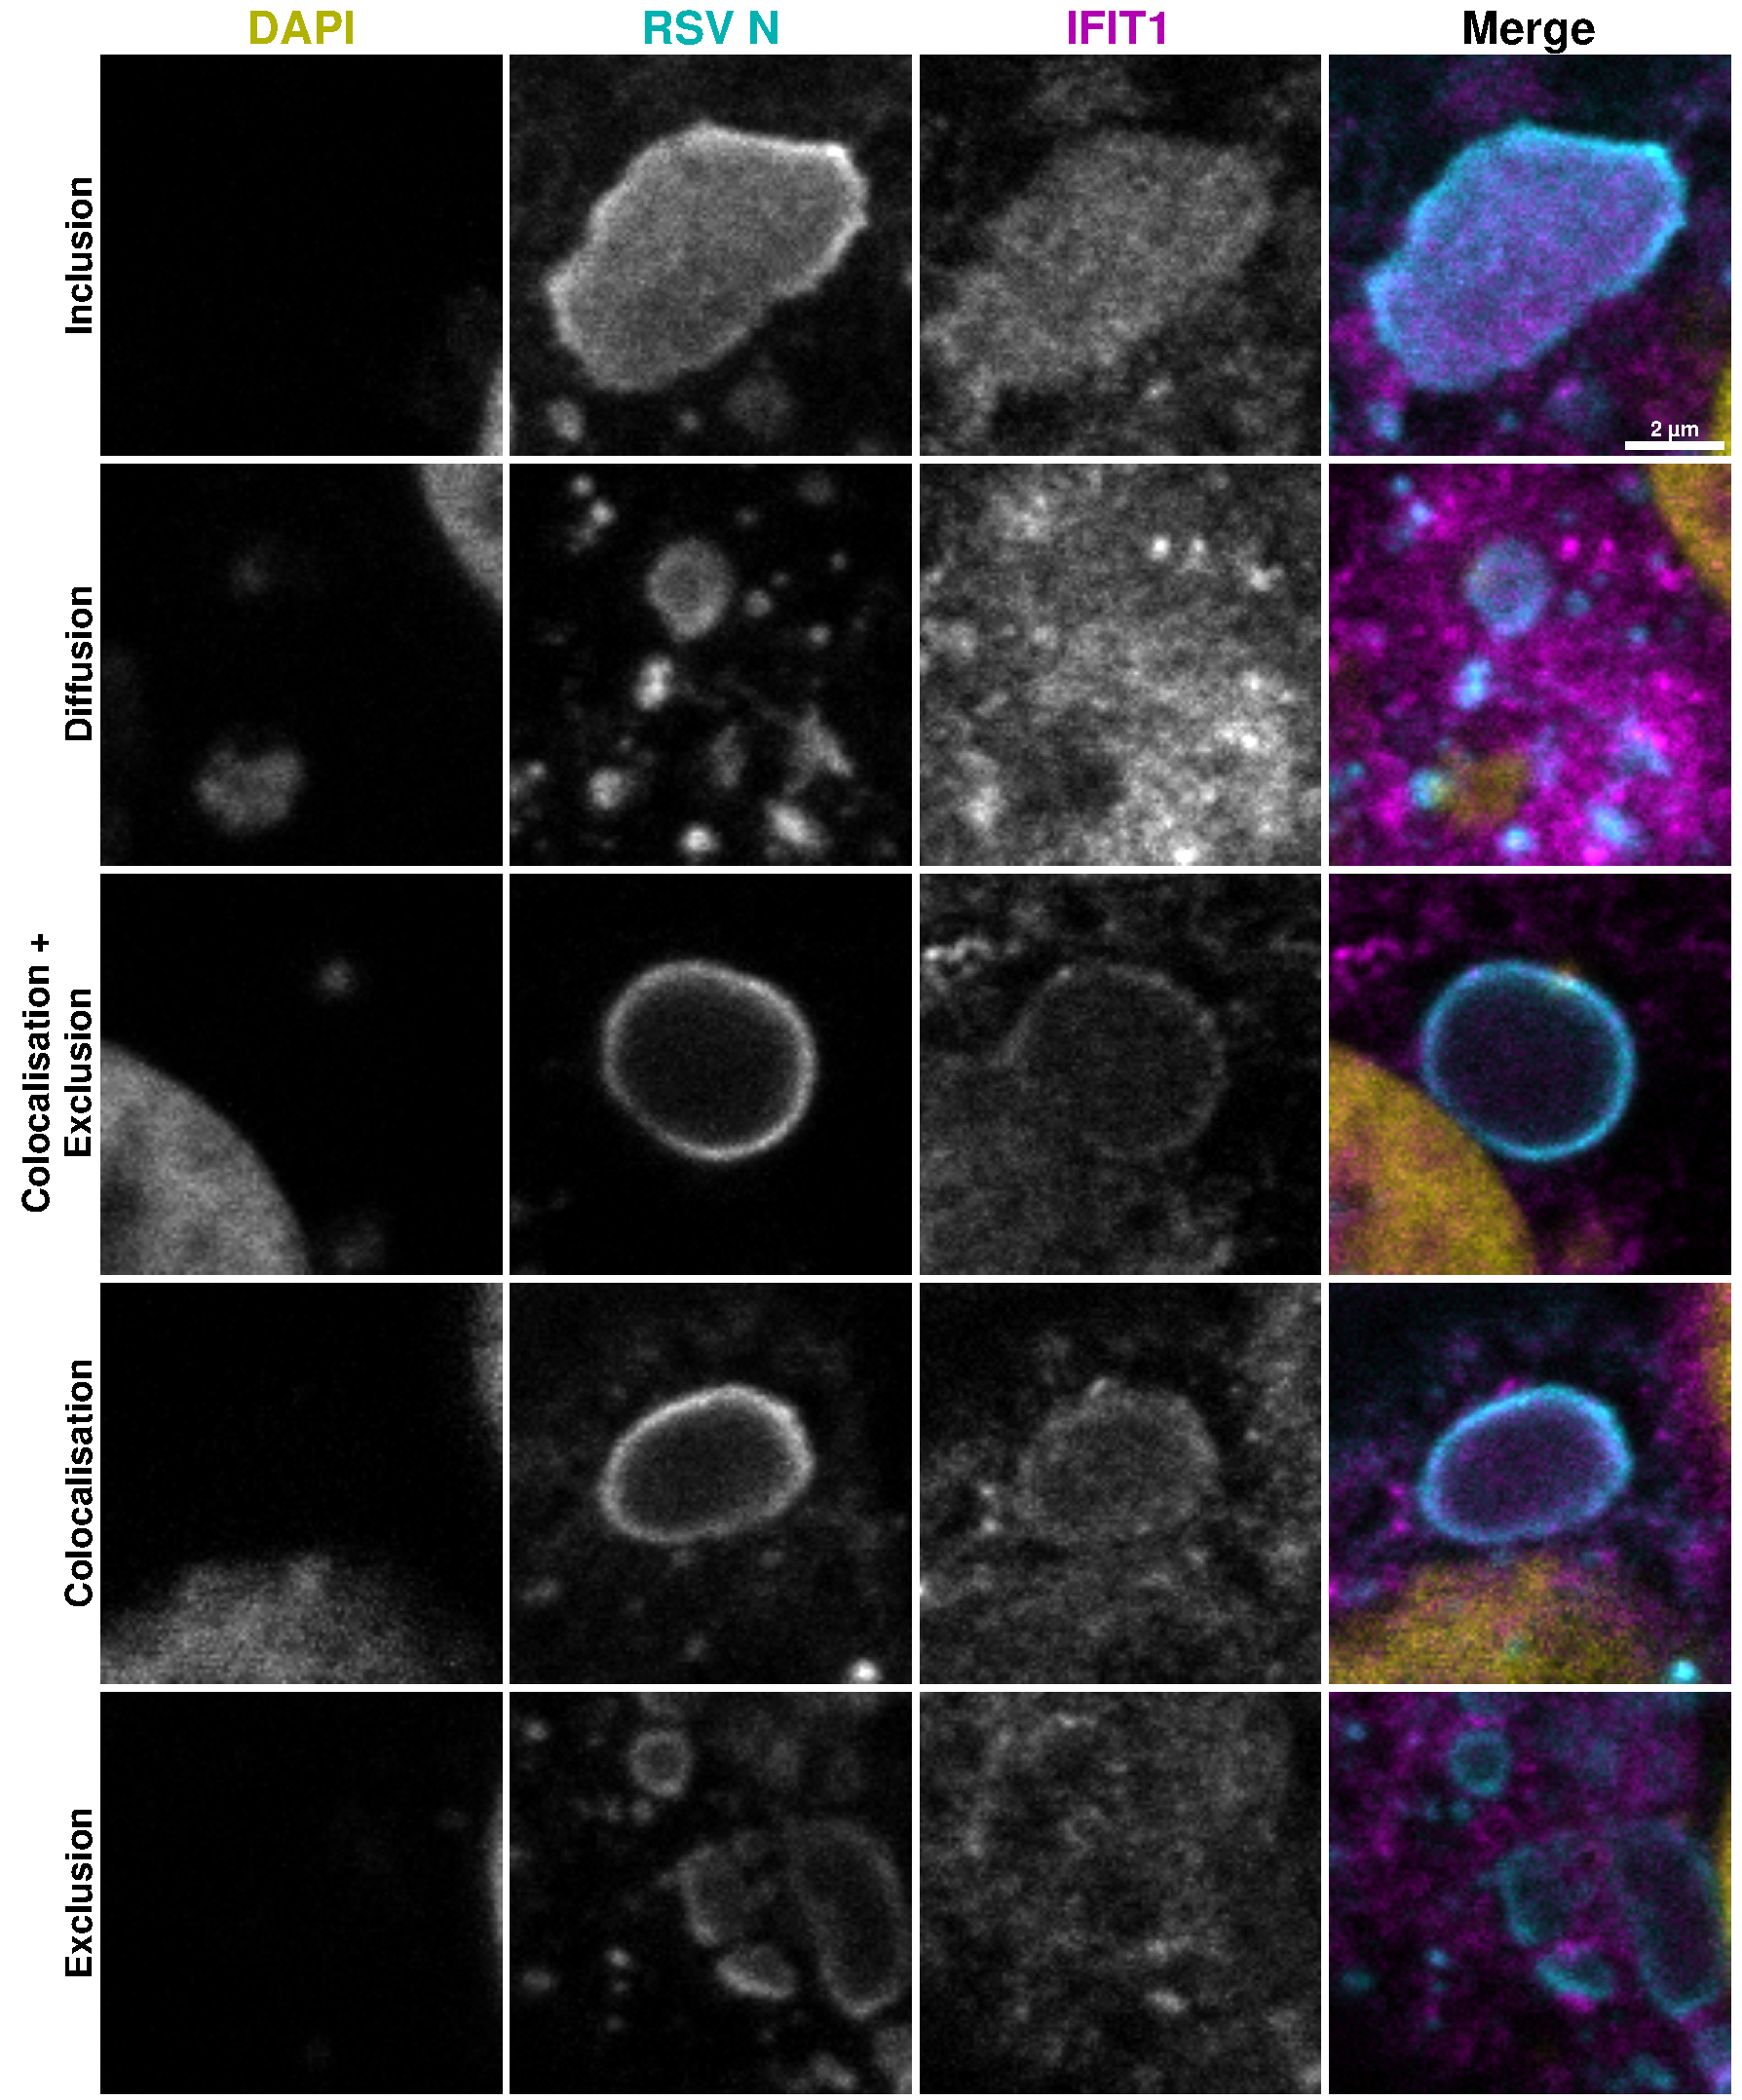
\includegraphics[width=1\linewidth]{09. Chapter 4/Figs/01. pIB/02. IFIT1/06. i1-vero-hnhp.pdf}
    \caption[Representative Images of Diverse Phenotypic Interactions of Monkey IFIT1 with Human Pseudo Inclusion Bodies (pIBs) in the VERO Cell Line.]{\textbf{Representative Images of Diverse Phenotypic Interactions of Monkey IFIT1 with Human Pseudo Inclusion Bodies (pIBs) in the VERO Cell Line.} Vero cells were transfected with hRSV N and P containing plasmids using TransIT-X2 and were fixed after 24 hours. Cellular nuclei were stained with DAPI (yellow), and cells were double-labeled with anti-RSV N (cyan) and anti-IFIT1 (magenta) antibodies. This figure showcases representative examples of relevant phenotypes in the interaction between monkey IFIT1 and hRSV pseudo inclusion bodies. These phenotypes are presented in descending order based on their percentage proportions. The scale bar indicates 2 \(\mu \mbox{m}\).}
    \label{fig:Representative Images of Diverse Phenotypic Interactions of Monkey IFIT1 with Human Pseudo Inclusion Bodies (pIBs) in the VERO Cell Line}
\end{figure}

43 38 8 5 5

2, 2, 9, 6, 1.1

In the context of bovine pIB structures, nascent monkey IFIT1 seems to colocalise with the edges of the structures (highlighted by the arrows). Consistent to human pIB data, nascent monkey IFIT1 is excluded from filamentous pIB network.

\begin{figure}
    \begin{subfigure}{0.495\textwidth}
        \caption{}
        \includegraphics[width=1\linewidth]{09. Chapter 4/Figs/01. pIB/02. IFIT1/07. bar_i1_vero_bnbp.pdf}  
    \end{subfigure}
    \begin{subfigure}{0.495\textwidth}
        \caption{}
        \includegraphics[width=1\linewidth]{09. Chapter 4/Figs/01. pIB/02. IFIT1/08. box_i1_vero_bnbp.pdf}
    \end{subfigure}
    \caption[Diverse Phenotypic Interactions of Monkey IFIT1 with Bovine Pseudo Inclusion Bodies (pIBs) in the VERO Cell Line.]{\textbf{Diverse Phenotypic Interactions of Monkey IFIT1 with Bovine Pseudo Inclusion Bodies (pIBs) in the VERO Cell Line.} Vero cells were transfected with bRSV N and P containing plasmids using TransIT-X2 and were fixed after 24 hours. Cells were labeled with anti-RSV N and anti-IFIT1 antibodies and imaged on confocal microscope. Panel (a) shows percentual proportions of observed phenotypes between bRSV pseudo inclusion bodies and monkey IFIT1 (14 observations), with the red dotted line denoting the 5\% threshold, marking phenotypes considered relevant above this limit. Panel (b) shows the IB area in \(\mu \mbox{m}^2\) per observed relevant phenotype.}
    \label{fig:Diverse Phenotypic Interactions of Monkey IFIT1 with Bovine Pseudo Inclusion Bodies (pIBs) in the VERO Cell Line}
\end{figure}

\begin{figure}
    \centering
    \includegraphics[width=1\linewidth]{09. Chapter 4/Figs/01. pIB/02. IFIT1/09. i1-vero-bnbp.pdf}
    \caption[Representative Images of Diverse Phenotypic Interactions of Monkey IFIT1 with Bovine Pseudo Inclusion Bodies (pIBs) in the VERO Cell Line.]{\textbf{Representative Images of Diverse Phenotypic Interactions of Monkey IFIT1 with Bovine Pseudo Inclusion Bodies (pIBs) in the VERO Cell Line.} Vero cells were transfected with bRSV N and P containing plasmids using TransIT-X2 and were fixed after 24 hours. Cellular nuclei were stained with DAPI (yellow), and cells were double-labeled with anti-RSV N (cyan) and anti-IFIT1 (magenta) antibodies. This figure showcases representative examples of relevant phenotypes in the interaction between monkey IFIT1 and bRSV pseudo inclusion bodies. These phenotypes are presented in descending order based on their percentage proportions. The scale bar indicates 2 \(\mu \mbox{m}\).}
    \label{fig:Representative Images of Diverse Phenotypic Interactions of Monkey IFIT1 with Bovine Pseudo Inclusion Bodies (pIBs) in the VERO Cell Line}
\end{figure}

56 44

1, 3

\subsubsection{Overexpressed Human IFIT1 During hRSV and bRSV Infection}
Overexpressed hIFIT1-FLAG colocalises with both human and bovine RSV IBs. This data is supported by evidence from z stacks.

\begin{figure}
    \begin{subfigure}{0.495\textwidth}
        \caption{}
        \includegraphics[width=1\linewidth]{09. Chapter 4/Figs/02. Overexpression/01. IFIT1/01. bar_i1_hrsv.pdf} 
    \end{subfigure}
    \begin{subfigure}{0.495\textwidth}
        \caption{}
        \includegraphics[width=1\linewidth]{09. Chapter 4/Figs/02. Overexpression/01. IFIT1/02. box_i1_hrsv.pdf}
    \end{subfigure}
    \caption[Observed Phenotypes of Exogenous hIFIT1 in the Context of hRSV Inclusion Bodies in VERO Cell Line.]{\textbf{Observed Phenotypes of Exogenous hIFIT1 in the Context of hRSV Inclusion Bodies in VERO Cell Line.} Vero cells were infected with human RSV at MOI 1. 24 HPI, the cells were transfected with hIFIT1-FLAG containing plasmids using TransIT-X2 and were fixed after further 24 hours. Cells were labeled with anti-RSV N and anti-FLAG antibodies and imaged on confocal microscope. Panel (a) shows percentual proportions of observed phenotypes between hRSV inclusion bodies and exogenous hIFIT1 (23 observations), with the red dotted line denoting the 5\% threshold, marking phenotypes considered relevant above this limit. Panel (b) shows the IB area in \(\mu \mbox{m}^2\) per observed relevant phenotype.}
    \label{fig:Observed Phenotypes of Exogenous hIFIT1 in the Context of hRSV Inclusion Bodies in VERO Cell Line}
\end{figure}

\begin{figure}
    \centering
    \includegraphics[width=1\linewidth]{09. Chapter 4/Figs/02. Overexpression/01. IFIT1/03. i1-hrsv.pdf}
    \caption[Representative Images of Observed Phenotypes of Exogenous hIFIT1 in the Context of hRSV Inclusion Bodies in VERO Cell Line.]{\textbf{Representative Images of Observed Phenotypes of Exogenous hIFIT1 in the Context of hRSV Inclusion Bodies in VERO Cell Line.} Vero cells were infected with human RSV at MOI 1. 24 HPI, the cells were transfected with hIFIT1-FLAG containing plasmids using TransIT-X2 and were fixed after further 24 hours. Cellular nuclei were stained with DAPI (yellow), and cells were double-labeled with anti-RSV N (cyan) and anti-FLAG (magenta) antibodies. This figure showcases representative examples of relevant phenotypes in the interaction between exogenous hIFIT1 and hRSV inclusion bodies. These phenotypes are presented in descending order based on their percentage proportions. The scale bar indicates 2 \(\mu \mbox{m}\).}
    \label{fig:Representative Images of Observed Phenotypes of Exogenous hIFIT1 in the Context of hRSV Inclusion Bodies in VERO Cell Line}
\end{figure}

74 21

1.1 2.2

\begin{figure}
    \begin{subfigure}{0.495\textwidth}
        \caption{}
        \includegraphics[width=1\linewidth]{09. Chapter 4/Figs/02. Overexpression/01. IFIT1/04. bar_i1_brsv.pdf} 
    \end{subfigure}
    \begin{subfigure}{0.495\textwidth}
        \caption{}
        \includegraphics[width=1\linewidth]{09. Chapter 4/Figs/02. Overexpression/01. IFIT1/05. box_i1_brsv.pdf}
    \end{subfigure}
    \caption[Observed Phenotypes of Exogenous hIFIT1 in the Context of bRSV Inclusion Bodies in VERO Cell Line.]{\textbf{Observed Phenotypes of Exogenous hIFIT1 in the Context of bRSV Inclusion Bodies in VERO Cell Line.} Vero cells were infected with bovine RSV at MOI 1. 24 HPI, the cells were transfected with hIFIT1-FLAG containing plasmids using TransIT-X2 and were fixed after further 24 hours. Cells were labeled with anti-RSV N and anti-FLAG antibodies and imaged on confocal microscope. Panel (a) shows percentual proportions of observed phenotypes between bRSV inclusion bodies and exogenous hIFIT1 (47 observations), with the red dotted line denoting the 5\% threshold, marking phenotypes considered relevant above this limit. Panel (b) shows the IB area in \(\mu \mbox{m}^2\) per observed relevant phenotype.}
    \label{fig:Observed Phenotypes of Exogenous hIFIT1 in the Context of bRSV Inclusion Bodies in VERO Cell Line}
\end{figure}

\begin{figure}
    \centering
    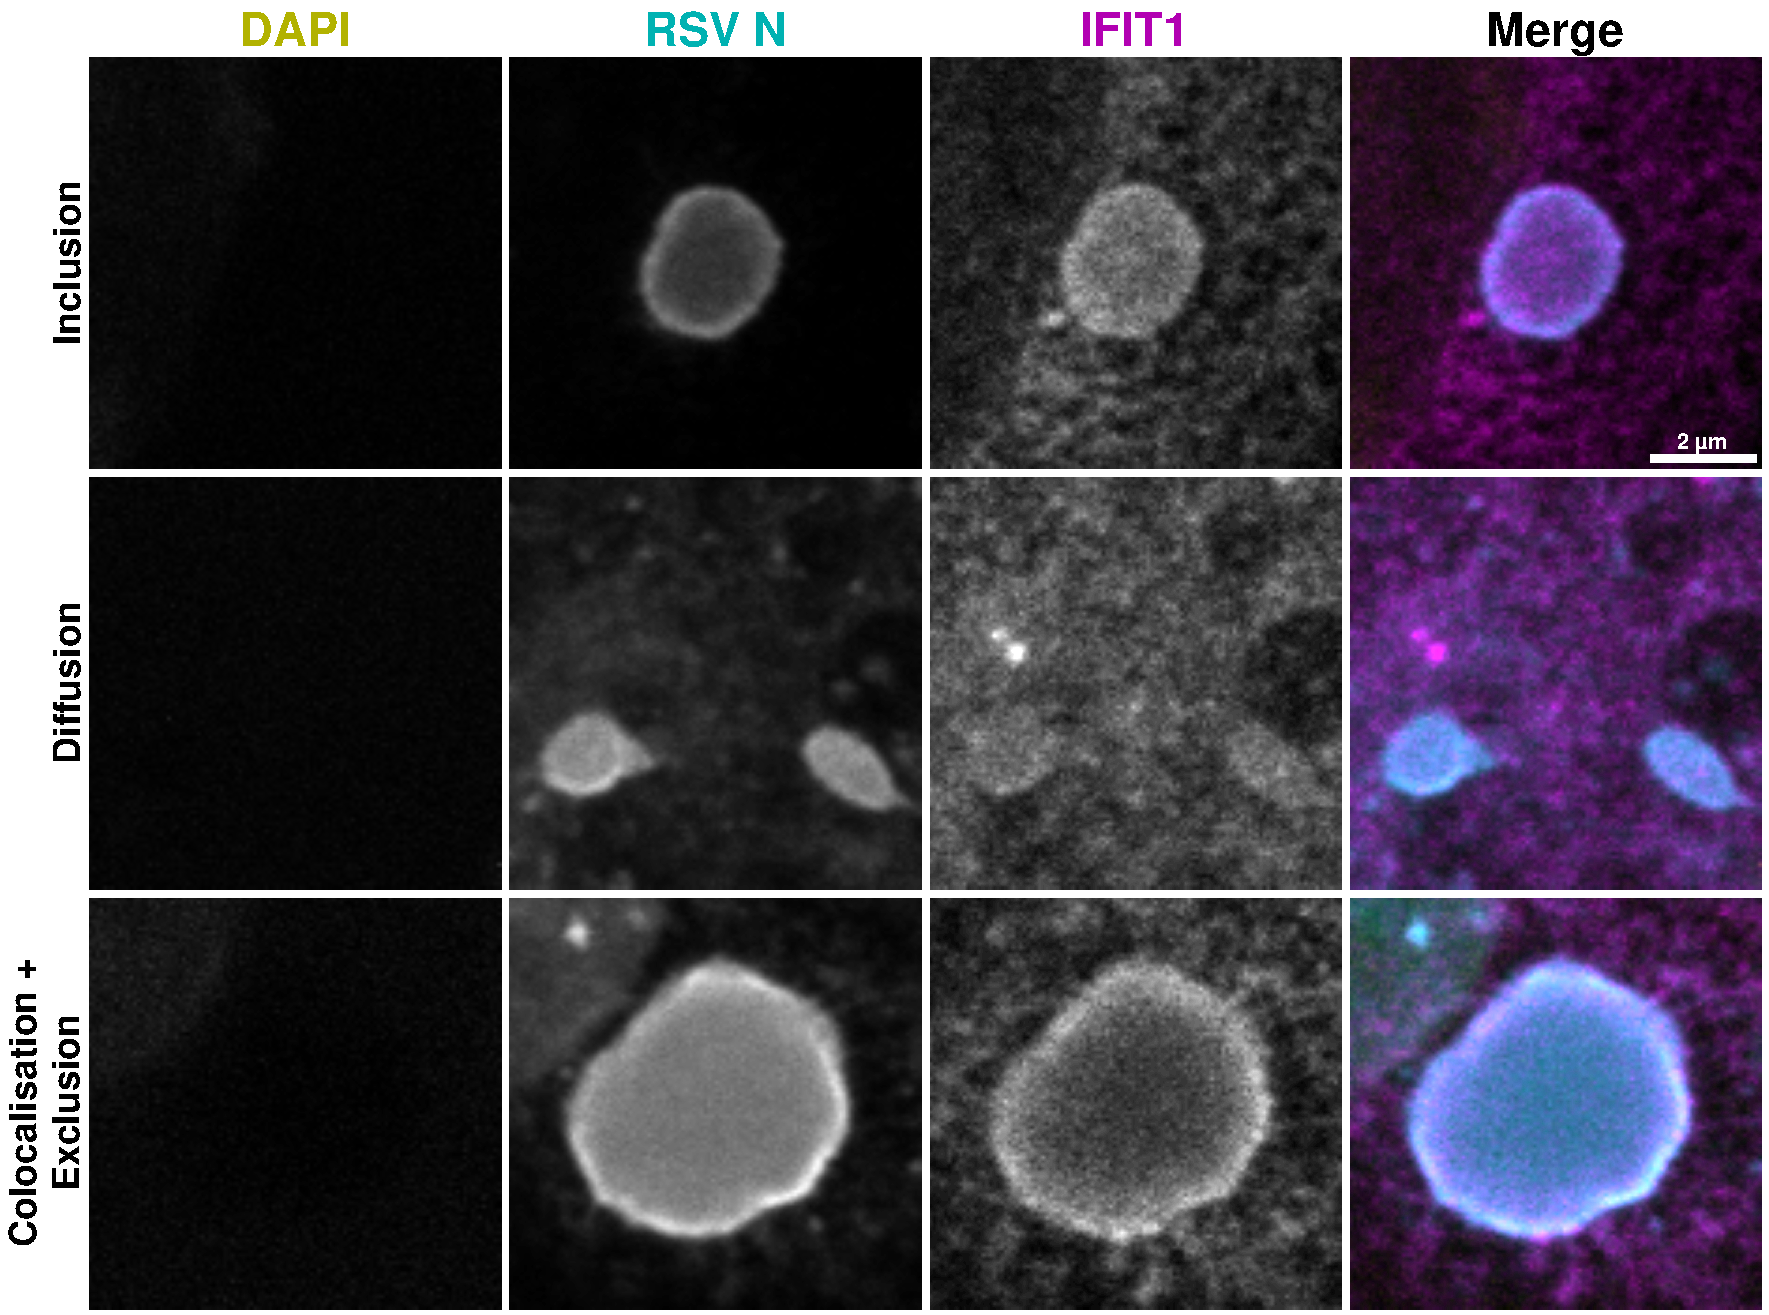
\includegraphics[width=1\linewidth]{09. Chapter 4/Figs/02. Overexpression/01. IFIT1/06. i1-brsv.pdf}
    \caption[Representative Images of Observed Phenotypes of Exogenous hIFIT1 in the Context of bRSV Inclusion Bodies in VERO Cell Line.]{\textbf{Representative Images of Observed Phenotypes of Exogenous hIFIT1 in the Context of bRSV Inclusion Bodies in VERO Cell Line.} Vero cells were infected with bovine RSV at MOI 1. 24 HPI, the cells were transfected with hIFIT1-FLAG containing plasmids using TransIT-X2 and were fixed after further 24 hours. Cellular nuclei were stained with DAPI (yellow), and cells were double-labeled with anti-RSV N (cyan) and anti-FLAG (magenta) antibodies. This figure showcases representative examples of relevant phenotypes in the interaction between exogenous hIFIT1 and bRSV inclusion bodies. These phenotypes are presented in descending order based on their percentage proportions. The scale bar indicates 2 \(\mu \mbox{m}\).}
    \label{fig:Representative Images of Observed Phenotypes of Exogenous hIFIT1 in the Context of bRSV Inclusion Bodies in VERO Cell Line}
\end{figure}

64 19 16

1.8, 0.8, 14

\subsubsection{Nascent Moneky IFIT3 and Its Interaction With pIBs}
Nascent monkey IFIT3 seems to behave a if he pIB was not here. This means I has diffused phenotype. One exception is the top panel (shown with the arrow) which hints at concentrated IFIT3 at the edge of the pIBs. We do not know the localisation with respect to the pIB filaments as none were found in the slides. This data is as well supported by z stack measurements.

\begin{figure}
    \begin{subfigure}{0.495\textwidth}
        \caption{}
        \includegraphics[width=1\linewidth]{09. Chapter 4/Figs/01. pIB/04. IFIT3/01. bar_i3_vero.pdf} 
    \end{subfigure}
    \begin{subfigure}{0.495\textwidth}
        \caption{}
        \includegraphics[width=1\linewidth]{09. Chapter 4/Figs/01. pIB/04. IFIT3/02. box_i3_vero.pdf}
    \end{subfigure}
    \caption[Diverse Phenotypic Interactions of Monkey IFIT3 with Human Pseudo Inclusion Bodies (pIBs) in the VERO Cell Line.]{\textbf{Diverse Phenotypic Interactions of Monkey IFIT3 with Human Pseudo Inclusion Bodies (pIBs) in the VERO Cell Line.} Vero cells were transfected with hRSV N and P containing plasmids using TransIT-X2 and were fixed after 24 hours. Cells were labeled with anti-RSV N and anti-IFIT3 antibodies and imaged on confocal microscope. Panel (a) shows percentual proportions of observed phenotypes between hRSV pseudo inclusion bodies and monkey IFIT3 (39 observations), with the red dotted line denoting the 5\% threshold, marking phenotypes considered relevant above this limit. Panel (b) shows the IB area in \(\mu \mbox{m}^2\) per observed relevant phenotype.}
    \label{fig:Diverse Phenotypic Interactions of Monkey IFIT3 with Human Pseudo Inclusion Bodies (pIBs) in the VERO Cell Line}
\end{figure}

\begin{figure}
    \centering
    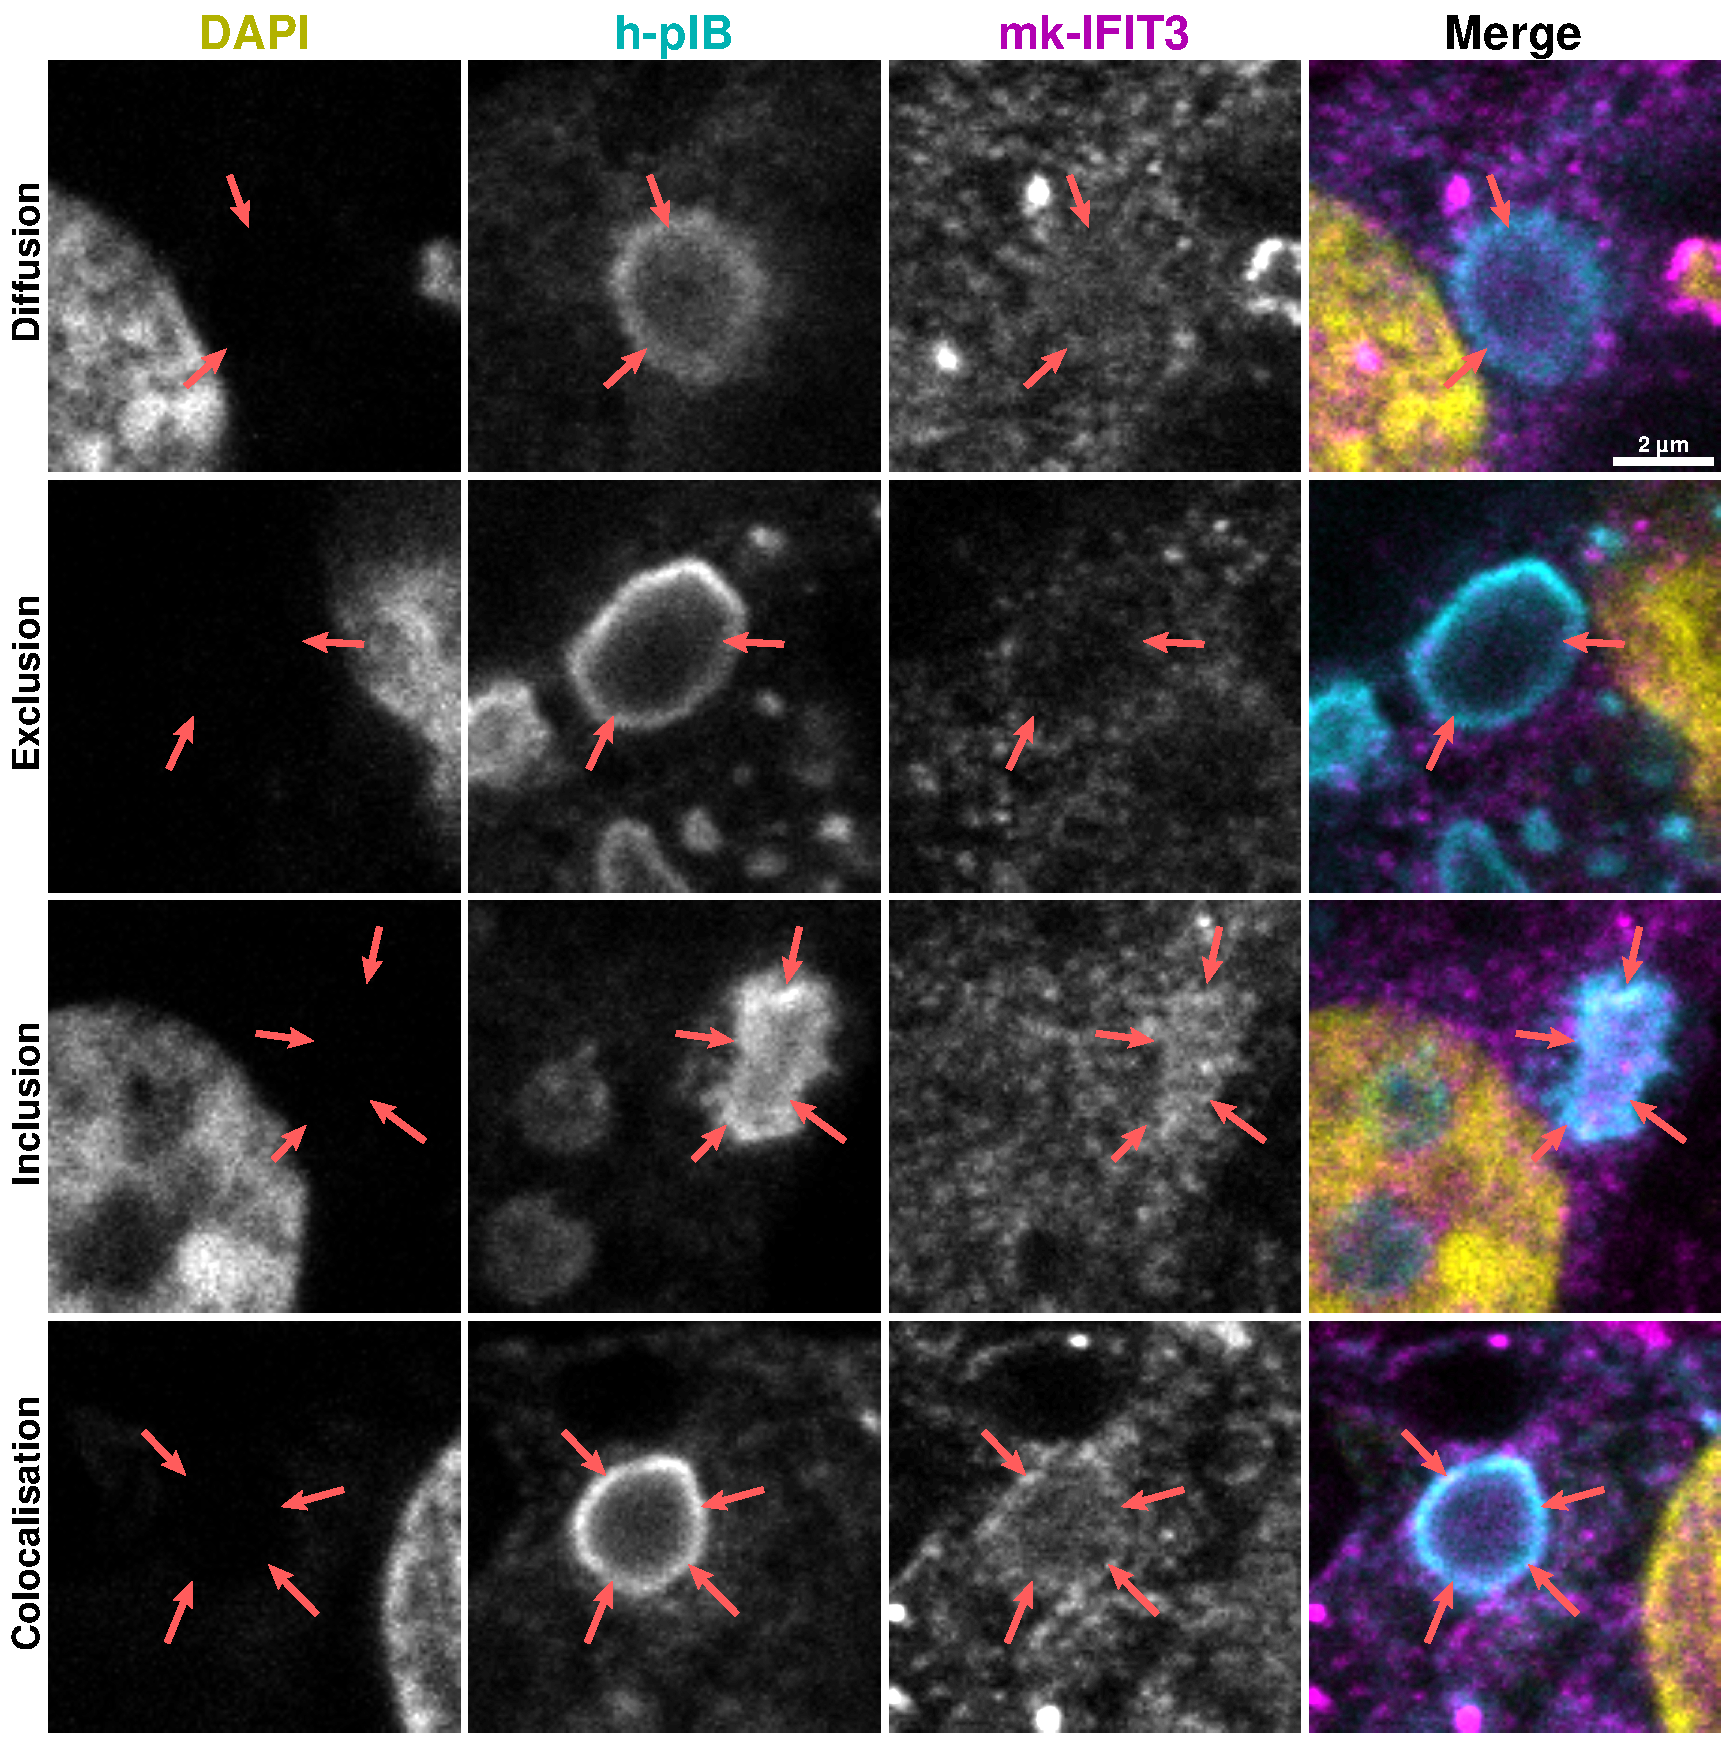
\includegraphics[width=1\linewidth]{09. Chapter 4/Figs/01. pIB/04. IFIT3/03. i3-vero-hnhp.pdf}
    \caption[Representative Images of Diverse Phenotypic Interactions of Monkey IFIT3 with Human Pseudo Inclusion Bodies (pIBs) in the VERO Cell Line.]{\textbf{Representative Images of Diverse Phenotypic Interactions of Monkey IFIT3 with Human Pseudo Inclusion Bodies (pIBs) in the VERO Cell Line.} Vero cells were transfected with hRSV N and P containing plasmids using TransIT-X2 and were fixed after 24 hours. Cellular nuclei were stained with DAPI (yellow), and cells were double-labeled with anti-RSV N (cyan) and anti-IFIT3 (magenta) antibodies. This figure showcases representative examples of relevant phenotypes in the interaction between monkey IFIT3 and hRSV pseudo inclusion bodies. These phenotypes are presented in descending order based on their percentage proportions. The scale bar indicates 2 \(\mu \mbox{m}\).}
    \label{fig:Representative Images of Diverse Phenotypic Interactions of Monkey IFIT3 with Human Pseudo Inclusion Bodies (pIBs) in the VERO Cell Line}
\end{figure}

41 36 15 5

4 2 4 3

\subsubsection{Overexpressed Bovine IFIT3 During hRSV and bRSV Infection}
Overexpressed bIFIT3-FLAG was observed to colocalise with hRSV inclusion bodies (top panel; highlighted with arrows), as well as being excluded from the hRSV IBs, without any signs of IFIT3 signal on the periphery of the IB structures (middle and bottom panel). This data is supported by z stack measurements.

\begin{figure}
    \begin{subfigure}{0.495\textwidth}
        \caption{}
        \includegraphics[width=1\linewidth]{09. Chapter 4/Figs/02. Overexpression/03. IFIT3/01. bar_i3_hrsv.pdf} 
    \end{subfigure}
    \begin{subfigure}{0.495\textwidth}
        \caption{}
        \includegraphics[width=1\linewidth]{09. Chapter 4/Figs/02. Overexpression/03. IFIT3/02. box_i3_hrsv.pdf}
    \end{subfigure}
    \caption[Observed Phenotypes of Exogenous bIFIT3 in the Context of hRSV Inclusion Bodies in VERO Cell Line.]{\textbf{Observed Phenotypes of Exogenous bIFIT3 in the Context of hRSV Inclusion Bodies in VERO Cell Line.} Vero cells were infected with human RSV at MOI 1. 24 HPI, the cells were transfected with bIFIT3-FLAG containing plasmids using TransIT-X2 and were fixed after further 24 hours. Cells were labeled with anti-RSV N and anti-FLAG antibodies and imaged on confocal microscope. Panel (a) shows percentual proportions of observed phenotypes between hRSV inclusion bodies and exogenous bIFIT3 (26 observations), with the red dotted line denoting the 5\% threshold, marking phenotypes considered relevant above this limit. Panel (b) shows the IB area in \(\mu \mbox{m}^2\) per observed relevant phenotype.}
    \label{fig:Observed Phenotypes of Exogenous bIFIT3 in the Context of hRSV Inclusion Bodies in VERO Cell Line}
\end{figure}

\begin{figure}
    \centering
    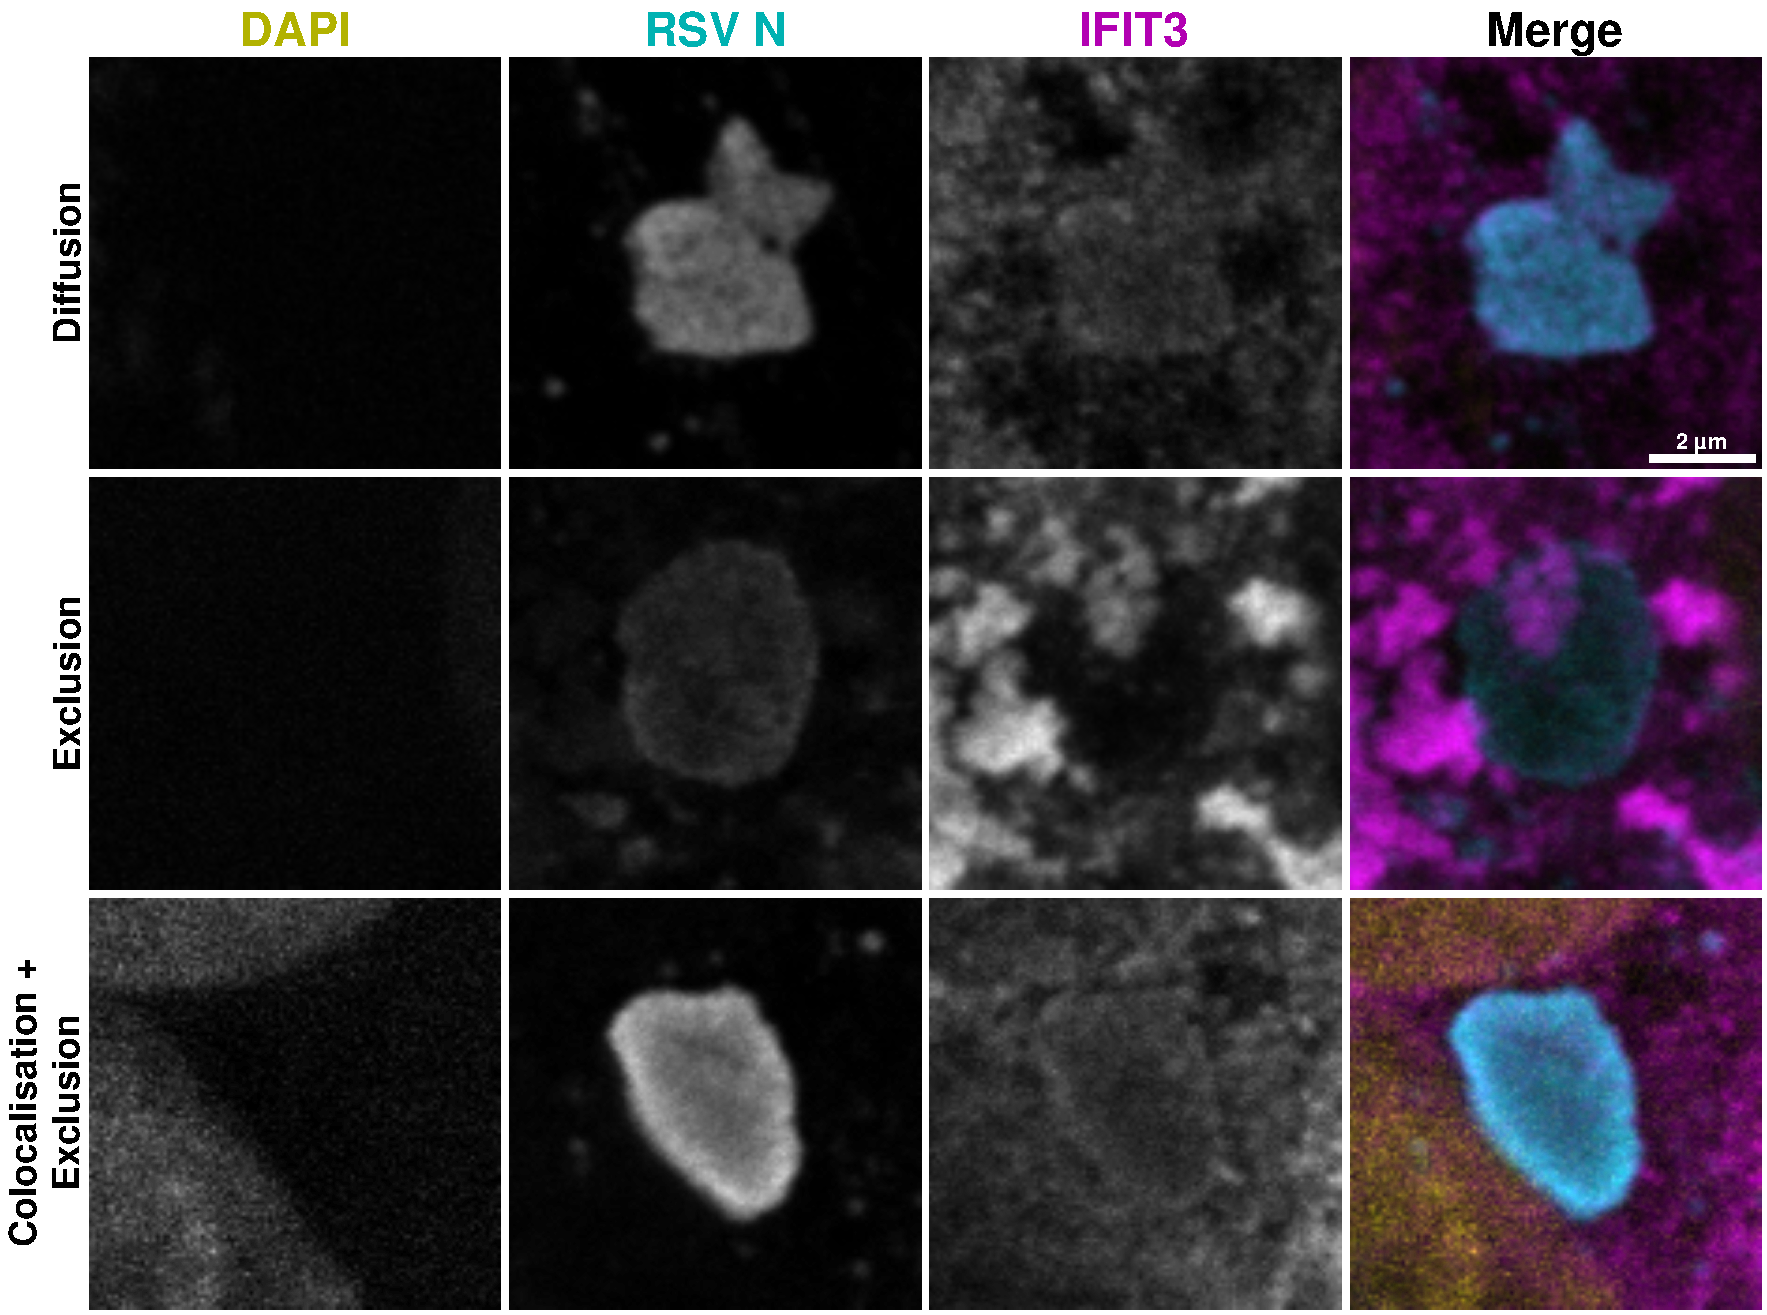
\includegraphics[width=1\linewidth]{09. Chapter 4/Figs/02. Overexpression/03. IFIT3/03. bi3-hrsv.pdf}
    \caption[Representative Images of Observed Phenotypes of Exogenous bIFIT3 in the Context of hRSV Inclusion Bodies in VERO Cell Line.]{\textbf{Representative Images of Observed Phenotypes of Exogenous bIFIT3 in the Context of hRSV Inclusion Bodies in VERO Cell Line.} Vero cells were infected with human RSV at MOI 1. 24 HPI, the cells were transfected with bIFIT3-FLAG containing plasmids using TransIT-X2 and were fixed after further 24 hours. Cellular nuclei were stained with DAPI (yellow), and cells were double-labeled with anti-RSV N (cyan) and anti-FLAG (magenta) antibodies. This figure showcases representative examples of relevant phenotypes in the interaction between exogenous bIFIT3 and hRSV inclusion bodies. These phenotypes are presented in descending order based on their percentage proportions. The scale bar indicates 2 \(\mu \mbox{m}\).}
    \label{fig:Representative Images of Observed Phenotypes of Exogenous bIFIT3 in the Context of hRSV Inclusion Bodies in VERO Cell Line}
\end{figure}

57 31 12

4, 3.3, 2.1

Very similar phenotype is observed for overexpressed bIFIT3-FLAG in bRSV infected cells. We see colocalization with IB (top panel) as well as exclusion from the structure without any signs of IFIT3 signal on the periphery of the IB structure (bottom panel). This data is as well supported by z stack measurements.

\begin{figure}
    \begin{subfigure}{0.495\textwidth}
        \caption{}
        \includegraphics[width=1\linewidth]{09. Chapter 4/Figs/02. Overexpression/03. IFIT3/04. bar_i3_brsv.pdf} 
    \end{subfigure}
    \begin{subfigure}{0.495\textwidth}
        \caption{}
        \includegraphics[width=1\linewidth]{09. Chapter 4/Figs/02. Overexpression/03. IFIT3/05. box_i3_brsv.pdf}
    \end{subfigure}
    \caption[Observed Phenotypes of Exogenous bIFIT3 in the Context of bRSV Inclusion Bodies in VERO Cell Line.]{\textbf{Observed Phenotypes of Exogenous bIFIT3 in the Context of bRSV Inclusion Bodies in VERO Cell Line.} Vero cells were infected with bovine RSV at MOI 1. 24 HPI, the cells were transfected with bIFIT3-FLAG containing plasmids using TransIT-X2 and were fixed after further 24 hours. Cells were labeled with anti-RSV N and anti-FLAG antibodies and imaged on confocal microscope. Panel (a) shows percentual proportions of observed phenotypes between bRSV inclusion bodies and exogenous bIFIT3 (13 observations), with the red dotted line denoting the 5\% threshold, marking phenotypes considered relevant above this limit. Panel (b) shows the IB area in \(\mu \mbox{m}^2\) per observed relevant phenotype.}
    \label{fig:Observed Phenotypes of Exogenous bIFIT3 in the Context of bRSV Inclusion Bodies in VERO Cell Line}
\end{figure}

\begin{figure}
    \centering
    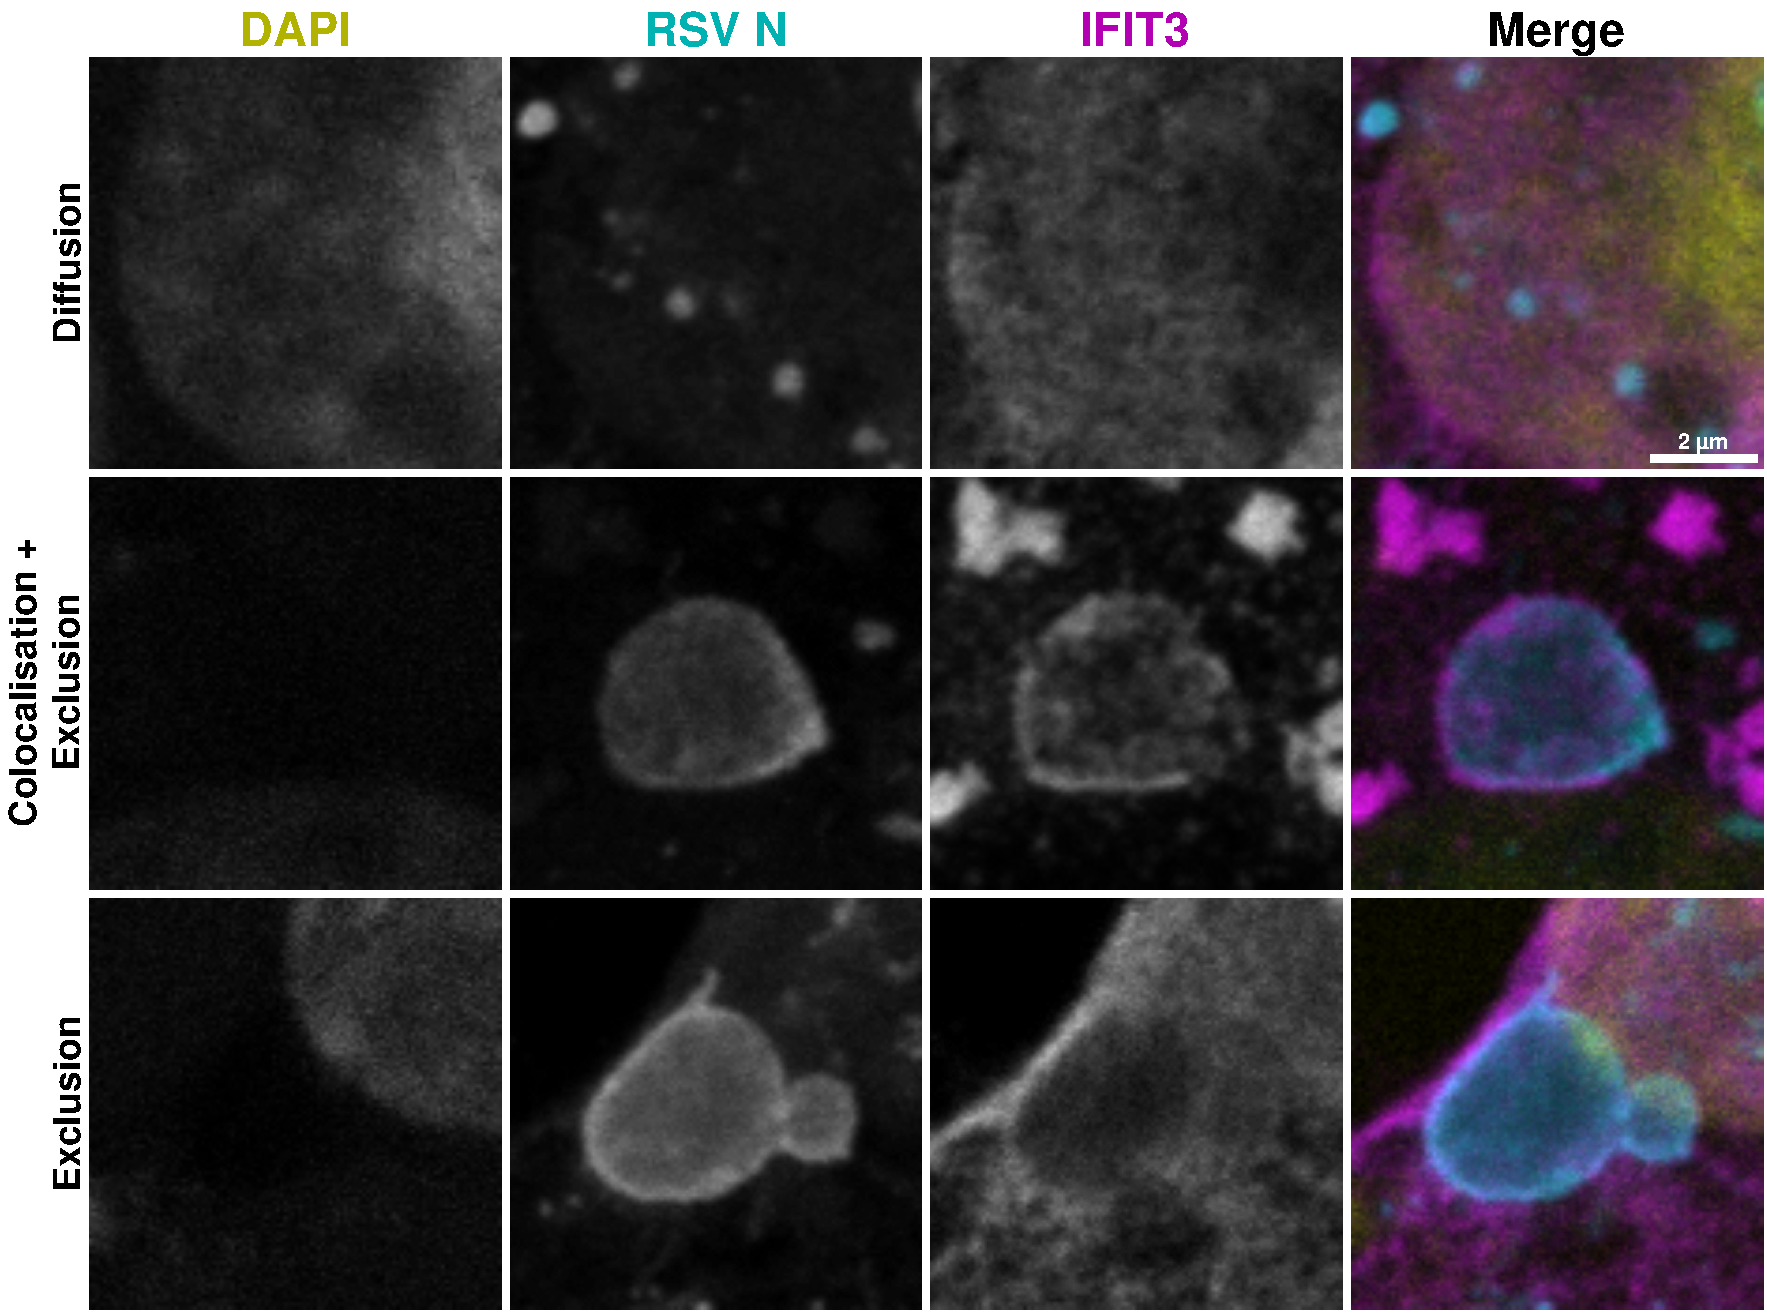
\includegraphics[width=1\linewidth]{09. Chapter 4/Figs/02. Overexpression/03. IFIT3/06. bi3-brsv.pdf}
    \caption[Representative Images of Observed Phenotypes of Exogenous bIFIT3 in the Context of bRSV Inclusion Bodies in VERO Cell Line.]{\textbf{Representative Images of Observed Phenotypes of Exogenous bIFIT3 in the Context of bRSV Inclusion Bodies in VERO Cell Line.} Vero cells were infected with bovine RSV at MOI 1. 24 HPI, the cells were transfected with bIFIT3-FLAG containing plasmids using TransIT-X2 and were fixed after further 24 hours. Cellular nuclei were stained with DAPI (yellow), and cells were double-labeled with anti-RSV N (cyan) and anti-FLAG (magenta) antibodies. This figure showcases representative examples of relevant phenotypes in the interaction between exogenous bIFIT3 and bRSV inclusion bodies. These phenotypes are presented in descending order based on their percentage proportions. The scale bar indicates 2 \(\mu \mbox{m}\).}
    \label{fig:Representative Images of Observed Phenotypes of Exogenous bIFIT3 in the Context of bRSV Inclusion Bodies in VERO Cell Line}
\end{figure}

54 31 15

0.22 0.9 6

\subsubsection{Nascent Moneky IFIT5 and Its Interaction With pIBs}
Nascent monkey IFIT5 colocalises with hRSV pseudo inclusion bodies (basically resembling the P staining). It also colocalises with pIB filamentous network. This network is only seen in cells that are co-transfected with RSV N and P proteins. We believe that they are an aftermath of a pIB breakdown. This data is as well supported by z stack measurements.

\begin{figure}
    \begin{subfigure}{0.495\textwidth}
        \caption{}
        \includegraphics[width=1\linewidth]{09. Chapter 4/Figs/01. pIB/05. IFIT5/01. bar_i5_vero.pdf} 
    \end{subfigure}
    \begin{subfigure}{0.495\textwidth}
        \caption{}
        \includegraphics[width=1\linewidth]{09. Chapter 4/Figs/01. pIB/05. IFIT5/02. box_i5_vero.pdf}
    \end{subfigure}
    \caption[Diverse Phenotypic Interactions of Monkey IFIT5 with Human Pseudo Inclusion Bodies (pIBs) in the VERO Cell Line.]{\textbf{Diverse Phenotypic Interactions of Monkey IFIT5 with Human Pseudo Inclusion Bodies (pIBs) in the VERO Cell Line.} Vero cells were transfected with hRSV N and P containing plasmids using TransIT-X2 and were fixed after 24 hours. Cells were labeled with anti-RSV N and anti-IFIT5 antibodies and imaged on confocal microscope. Panel (a) shows percentual proportions of observed phenotypes between hRSV pseudo inclusion bodies and monkey IFIT5 (100 observations), with the red dotted line denoting the 5\% threshold, marking phenotypes considered relevant above this limit. Panel (b) shows the IB area in \(\mu \mbox{m}^2\) per observed relevant phenotype.}
    \label{fig:Diverse Phenotypic Interactions of Monkey IFIT5 with Human Pseudo Inclusion Bodies (pIBs) in the VERO Cell Line}
\end{figure}

\begin{figure}
    \centering
    \includegraphics[width=1\linewidth]{09. Chapter 4/Figs/01. pIB/05. IFIT5/03. i5-vero-hnhp.pdf}
    \caption[Representative Images of Diverse Phenotypic Interactions of Monkey IFIT5 with Human Pseudo Inclusion Bodies (pIBs) in the VERO Cell Line.]{\textbf{Representative Images of Diverse Phenotypic Interactions of Monkey IFIT5 with Human Pseudo Inclusion Bodies (pIBs) in the VERO Cell Line.} Vero cells were transfected with hRSV N and P containing plasmids using TransIT-X2 and were fixed after 24 hours. Cellular nuclei were stained with DAPI (yellow), and cells were double-labeled with anti-RSV N (cyan) and anti-IFIT5 (magenta) antibodies. This figure showcases representative examples of relevant phenotypes in the interaction between monkey IFIT5 and hRSV pseudo inclusion bodies. These phenotypes are presented in descending order based on their percentage proportions. The scale bar indicates 2 \(\mu \mbox{m}\).}
    \label{fig:Representative Images of Diverse Phenotypic Interactions of Monkey IFIT5 with Human Pseudo Inclusion Bodies (pIBs) in the VERO Cell Line}
\end{figure}

62 38

1.2 4

\subsubsection{Overexpressed Human IFIT5 During hRSV and bRSV Infection}
hIFIT5-FLAG is colocalising with hRSV inclusion bodies (basically resembling the P staining), while in bRSV infected cell there is a hint of IFIT5 signal concentration at the side of bRSV IB.

This data is by single cells per conditions as transfection did not work well. It is however supported by z stack measurements.

\begin{figure}
    \begin{subfigure}{0.495\textwidth}
        \caption{}
        \includegraphics[width=1\linewidth]{09. Chapter 4/Figs/02. Overexpression/04. IFIT5/01. bar_i5_hrsv.pdf} 
    \end{subfigure}
    \begin{subfigure}{0.495\textwidth}
        \caption{}
        \includegraphics[width=1\linewidth]{09. Chapter 4/Figs/02. Overexpression/04. IFIT5/02. box_i5_hrsv.pdf}
    \end{subfigure}
    \caption[Observed Phenotypes of Exogenous hIFIT5 in the Context of hRSV Inclusion Bodies in VERO Cell Line.]{\textbf{Observed Phenotypes of Exogenous hIFIT5 in the Context of hRSV Inclusion Bodies in VERO Cell Line.} Vero cells were infected with human RSV at MOI 1. 24 HPI, the cells were transfected with hIFIT5-FLAG containing plasmids using TransIT-X2 and were fixed after further 24 hours. Cells were labeled with anti-RSV N and anti-FLAG antibodies and imaged on confocal microscope. Panel (a) shows percentual proportions of observed phenotypes between hRSV inclusion bodies and exogenous hIFIT5 (11 observations), with the red dotted line denoting the 5\% threshold, marking phenotypes considered relevant above this limit. Panel (b) shows the IB area in \(\mu \mbox{m}^2\) per observed relevant phenotype.}
    \label{fig:Observed Phenotypes of Exogenous hIFIT5 in the Context of hRSV Inclusion Bodies in VERO Cell Line}
\end{figure}

\begin{figure}
    \centering
    \includegraphics[width=1\linewidth]{09. Chapter 4/Figs/02. Overexpression/04. IFIT5/03. i5-hrsv.pdf}
    \caption[Representative Images of Observed Phenotypes of Exogenous hIFIT5 in the Context of hRSV Inclusion Bodies in VERO Cell Line.]{\textbf{Representative Images of Observed Phenotypes of Exogenous hIFIT5 in the Context of hRSV Inclusion Bodies in VERO Cell Line.} Vero cells were infected with human RSV at MOI 1. 24 HPI, the cells were transfected with hIFIT5-FLAG containing plasmids using TransIT-X2 and were fixed after further 24 hours. Cellular nuclei were stained with DAPI (yellow), and cells were double-labeled with anti-RSV N (cyan) and anti-FLAG (magenta) antibodies. This figure showcases representative examples of relevant phenotypes in the interaction between exogenous hIFIT5 and hRSV inclusion bodies. These phenotypes are presented in descending order based on their percentage proportions. The scale bar indicates 2 \(\mu \mbox{m}\).}
    \label{fig:Representative Images of Observed Phenotypes of Exogenous hIFIT5 in the Context of hRSV Inclusion Bodies in VERO Cell Line}
\end{figure}

45 26 26

0.7 1.2 6

\begin{figure}
    \begin{subfigure}{0.495\textwidth}
        \caption{}
        \includegraphics[width=1\linewidth]{09. Chapter 4/Figs/02. Overexpression/04. IFIT5/04. bar_i5_brsv.pdf} 
    \end{subfigure}
    \begin{subfigure}{0.495\textwidth}
        \caption{}
        \includegraphics[width=1\linewidth]{09. Chapter 4/Figs/02. Overexpression/04. IFIT5/05. box_i5_brsv.pdf}
    \end{subfigure}
    \caption[Observed Phenotypes of Exogenous hIFIT5 in the Context of bRSV Inclusion Bodies in VERO Cell Line.]{\textbf{Observed Phenotypes of Exogenous hIFIT5 in the Context of bRSV Inclusion Bodies in VERO Cell Line.} Vero cells were infected with bovine RSV at MOI 1. 24 HPI, the cells were transfected with hIFIT5-FLAG containing plasmids using TransIT-X2 and were fixed after further 24 hours. Cells were labeled with anti-RSV N and anti-FLAG antibodies and imaged on confocal microscope. Panel (a) shows percentual proportions of observed phenotypes between bRSV inclusion bodies and exogenous hIFIT5 (5 observations), with the red dotted line denoting the 5\% threshold, marking phenotypes considered relevant above this limit. Panel (b) shows the IB area in \(\mu \mbox{m}^2\) per observed relevant phenotype.}
    \label{fig:Observed Phenotypes of Exogenous hIFIT5 in the Context of bRSV Inclusion Bodies in VERO Cell Line}
\end{figure}

\begin{figure}
    \centering
    \includegraphics[width=1\linewidth]{09. Chapter 4/Figs/02. Overexpression/04. IFIT5/06. i5-brsv.pdf}
    \caption[Representative Images of Observed Phenotypes of Exogenous hIFIT5 in the Context of bRSV Inclusion Bodies in VERO Cell Line.]{\textbf{Representative Images of Observed Phenotypes of Exogenous hIFIT5 in the Context of bRSV Inclusion Bodies in VERO Cell Line.} Vero cells were infected with bovine RSV at MOI 1. 24 HPI, the cells were transfected with hIFIT5-FLAG containing plasmids using TransIT-X2 and were fixed after further 24 hours. Cellular nuclei were stained with DAPI (yellow), and cells were double-labeled with anti-RSV N (cyan) and anti-FLAG (magenta) antibodies. This figure showcases representative examples of relevant phenotypes in the interaction between exogenous hIFIT5 and bRSV inclusion bodies. These phenotypes are presented in descending order based on their percentage proportions. The scale bar indicates 2 \(\mu \mbox{m}\).}
    \label{fig:Representative Images of Observed Phenotypes of Exogenous hIFIT5 in the Context of bRSV Inclusion Bodies in VERO Cell Line}
\end{figure}

80 20

0.7 2.5

% summary
Overexpressed hIFIT1-FLAG in the context of h/bRSV infection colocalises to both human and bovine IB structures.

Overexpressed bIFIT3 behaves equally between hRSV and bRSV infection, that is it sometimes colocalises with the IB structure and sometimes is completely excluded from the structure.

Overexpressed hIFIT5 in hRSV infected cells colocalises with the IBs.
